% witness: synthetic (revRG1 B1 in a tikz node; text-width nodes as 2410.06985's; the second node revRG1b B1, a
%          group of glue)
% oracle:  pdflatex 0 errors: a one-line node "x", 11.37149pt high as `\hbox{\tikz\node…}` (ours RG1b 11.37155pt,
%          rg1 23.37155pt), the picture's 15.73 (11.37pt in px)
% engines: rust rg1 = <picture height="32.34">, foreignObject depth 1.2em (an empty line under x); int162a = 15.73, 0em;
%          the second node `{x{\quad\par}}`: rg1b 32.34 and 1.2em, int162a 15.73 and 0em
% expect:  0 errors, 0 warnings; both <picture height="15.73">, foreignObject height 5.96, depth 0em; each node's
%          empty first <p/> is int162a's too (not this mechanism; cause not traced)
% status:  RED (rg1) -> GREEN (RG1b); the second node RED (rg1b) -> GREEN (RG1c)
\documentclass{article}
\usepackage{tikz}
\begin{document}
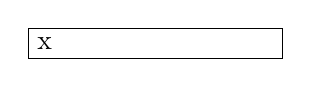
\begin{tikzpicture}
\node[draw, text width=3cm] {x{ \par}};
\end{tikzpicture}

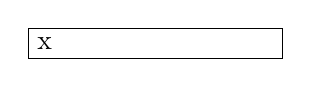
\begin{tikzpicture}
\node[draw, text width=3cm] {x{\quad\par}};
\end{tikzpicture}
\end{document}
